\subsubsection{Componentes}
% Motor: 
% https://www.pololu.com/product/2212
% https://www.pololu.com/product/2212
% Encoder:
% https://www.pololu.com/product/3081
% Driver motor:
% https://www.pololu.com/product/713
% ESP32:

São quatro o número de componentes básicos que compõem os robôs presentes neste trabalho, sendo eles: um par de atuadores (motor direito e esquerdo), um par de sensores de rotação (\textit{Encoder}s magnéticos), um driver motor multicanal, um microcontrolador e bateria recarregável. Devido as características dos componentes escolhidos para o projeto, apenas estes quatro tipos foram suficiente para compor a eletrônica do robô de forma a respeitar as restrições dimensionais, realizar o controle feedforward/backward de forma eficiência e com um bom período de amostragem e baixo gasto energético, além de um baixo custo financeiro.

A seguir serão apresentados mais detalhes dos componentes supracitados.

% 30:1 Micro Metal Gearmotor HP 6V with Extended Motor Shaft
\begin{figure}[H]
    \centering
    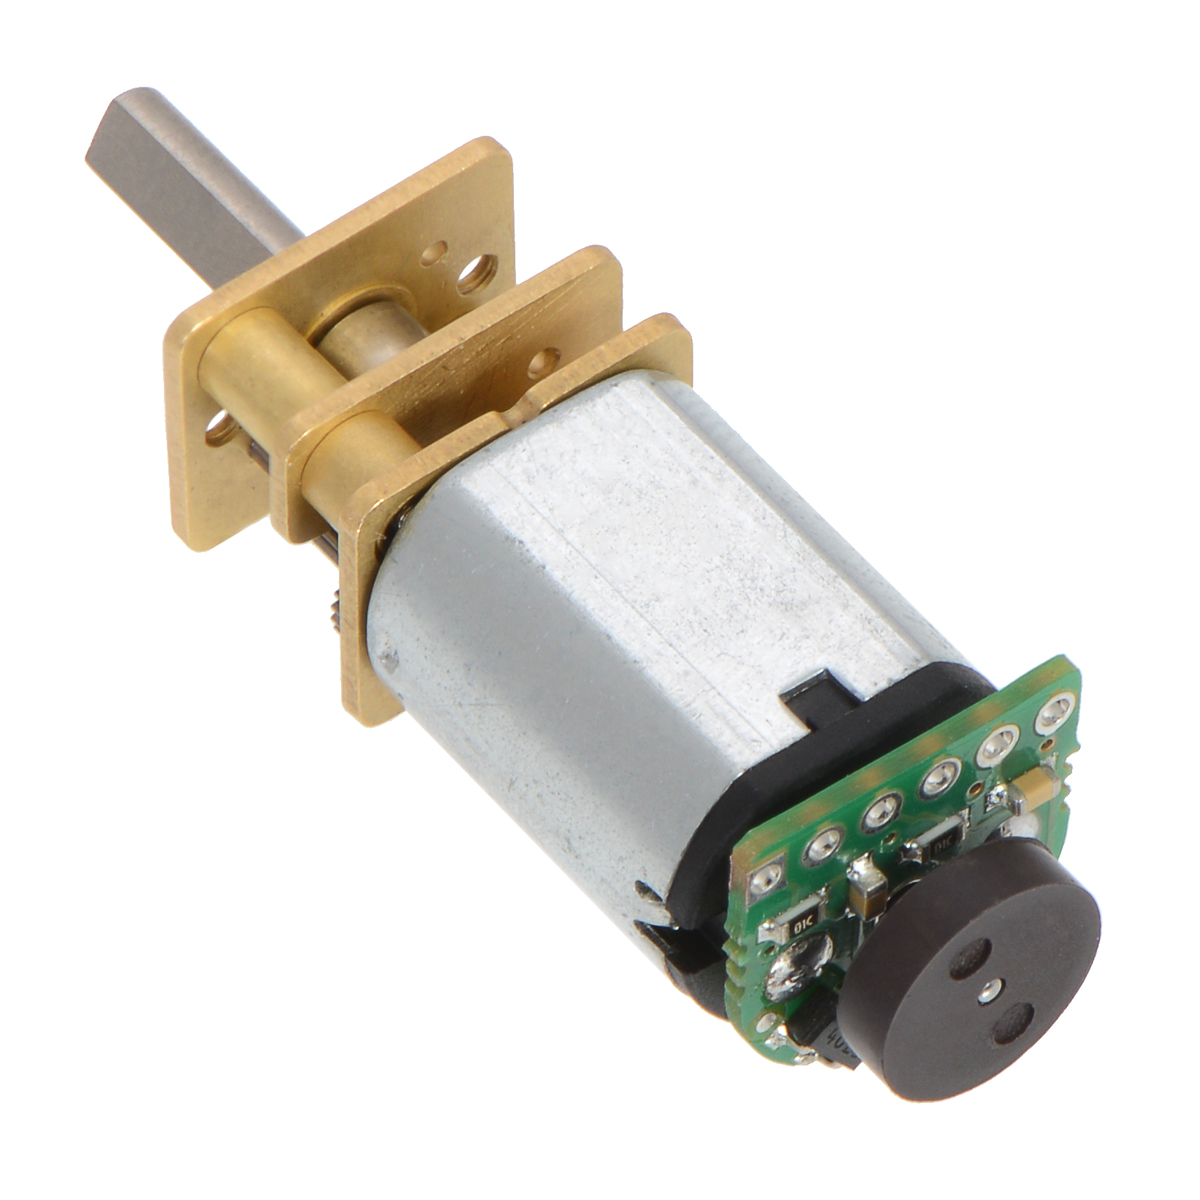
\includegraphics[width=3cm]{imagens/eletronica/motor_com_encoder.jpg}
    \caption{Micro Motor de 6V com caixa de redução de 30:1 e \textit{Encoder} magnético.}
    \label{fig:motor_com_encoder}
\end{figure}

A figura \ref{fig:motor_com_encoder} mostra o motor escolhido já com o \textit{Encoder} magnético colocado em seu eixo estendido (placa de circuito impresso com um Imã natural em forma de disco), esse é um micro motor de $6$V com uma caixa de redução de $\approx 30:1$ da \textit{Pololu}[?].

\begin{figure}[H]
    \centering
    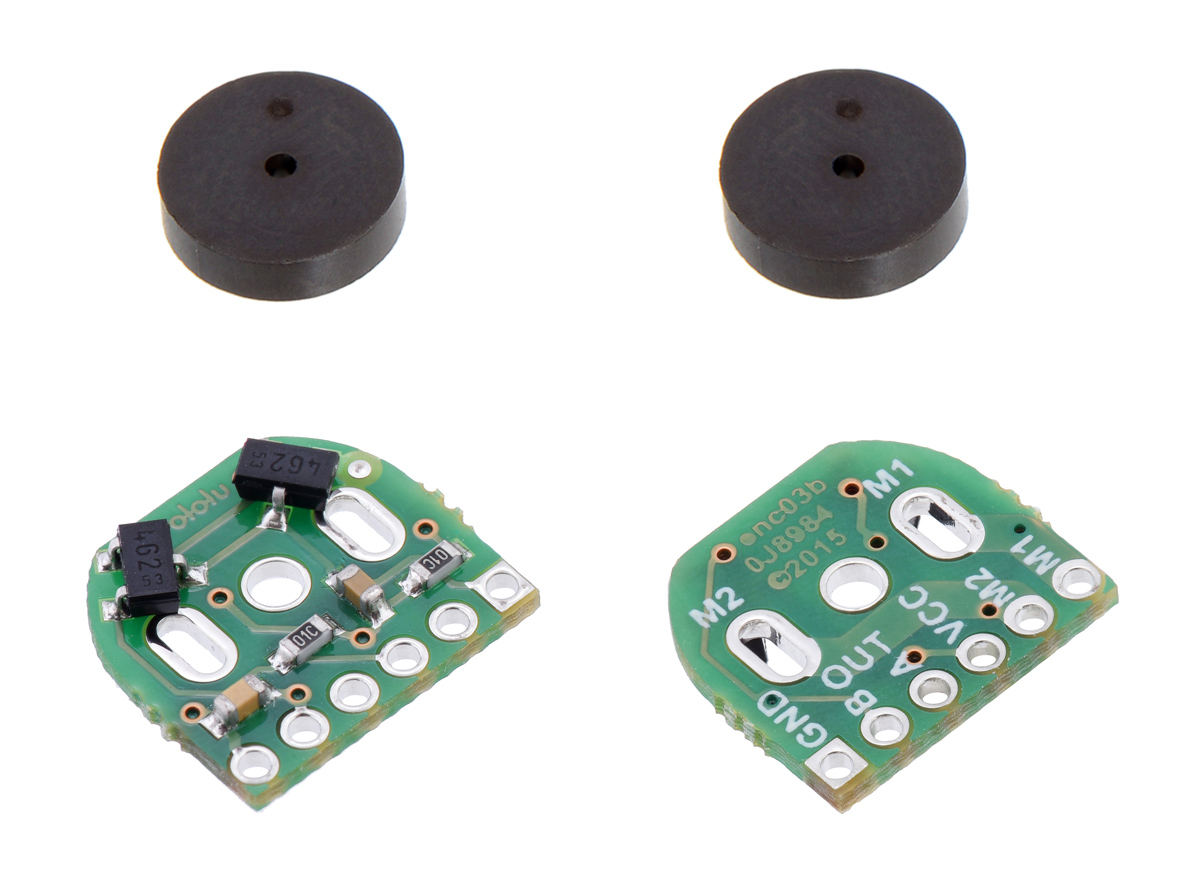
\includegraphics[width=5cm]{imagens/eletronica/encoder_frente_verso.jpg}
    \caption{Par de Encoders Magnéticos de $12$ pulsos por revolução ($12$CPR)}
    \label{fig:encoder}
\end{figure}

\begin{figure}[H]
    \centering
    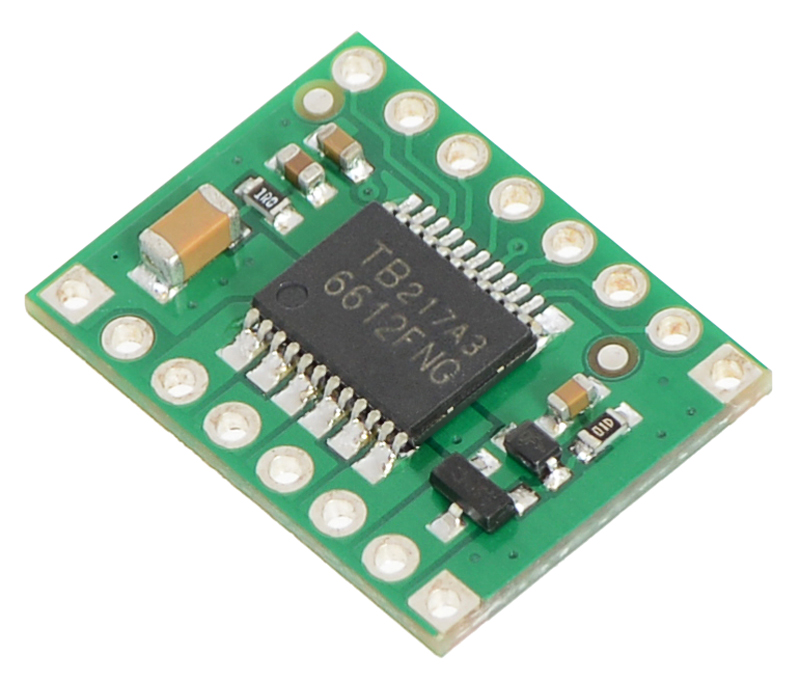
\includegraphics[width=3cm]{imagens/eletronica/driver.jpg}
    \caption{\textit{Driver} Motor TB6612FNG.}
    \label{fig:driver_motor}
\end{figure}

\begin{figure}[H]
    \centering
    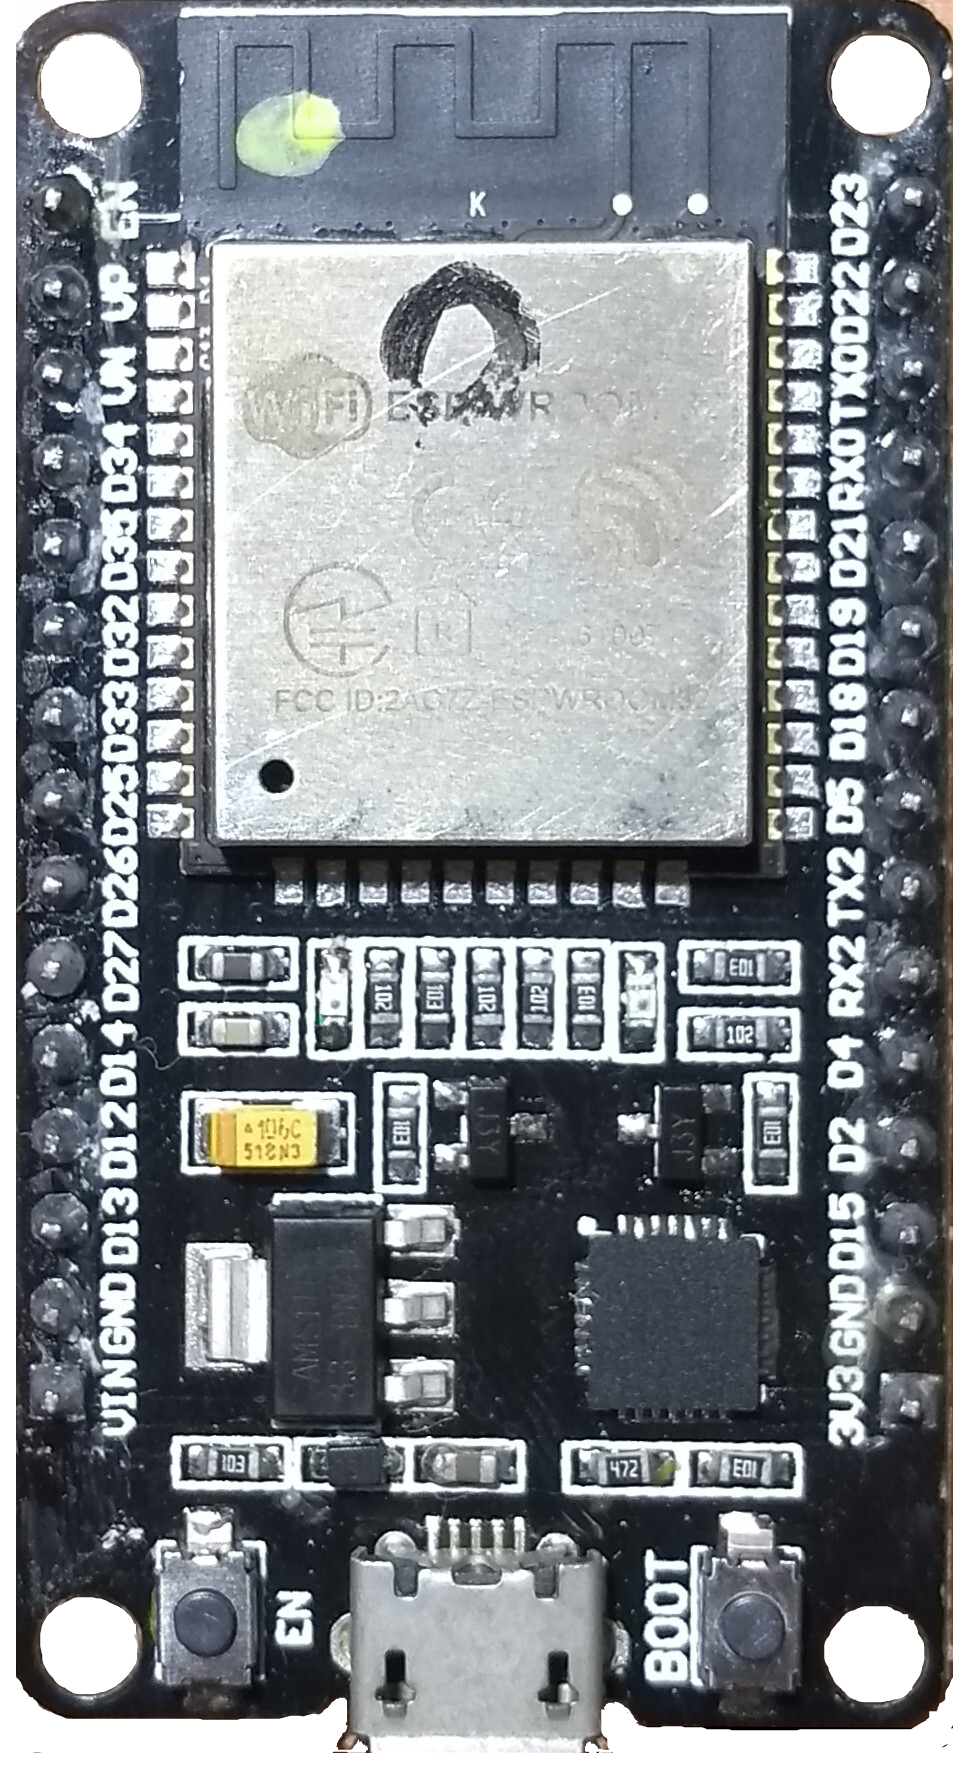
\includegraphics[width=3cm]{imagens/eletronica/esp32_kit.png}
    \caption{Placa de desenvolvimento ESP32 Dev1.}
    \label{fig:esp32_kit}
\end{figure}